\chapter{Xarxa Neuronal}
\section{Introducció}
En iniciar la part pràctica del treball vam decidir crear tres tipus de xarxes neuronals: una \nameref{sec:10}, una altra \nameref{sec:11} i, finalment, una \nameref{sec:12}.

En aquest capítol explicarem com vam elaborar cadascuna d’aquestes xarxes neuronals i, a més, compararem les dues formes de desenvolupament en una \nameref{sec:op}.

Per facilitar l’organització del treball, ens hem repartit les tasques: un membre de l’equip s’ha encarregat de la xarxa neuronal implementada amb llenguatge de programació, mentre que l’altre ha treballat amb la xarxa neuronal feta amb fulls de càlcul. Finalment, hem elaborat conjuntament la taula de comparació, intercanviant perspectives, i també hem treballat plegats la xarxa neuronal del cas real.



\section{Xarxa neuronal de regressió}\label{sec:op}
Una intel·ligència artificial és un camp molt extens i, dins d’aquest, les xarxes neuronals també representen una branca àmplia i complexa.
En el nostre context utilitzarem un tipus concret de xarxa neuronal per a la pràctica: les \textbf{xarxes neuronals de regressió}.

Una xarxa neuronal de regressió, a diferència d’una de classificació, té una sortida de tipus lineal que permet predir un valor numèric continu. Aquest tipus de xarxes requereixen un conjunt de dades prou extens i ben estructurat per poder aprendre les relacions entre les variables d’entrada i generar una estimació fiable.

A continuació es mostra un esquema representatiu d’una xarxa neuronal de regressió:

\begin{figure}[h!]
\centering
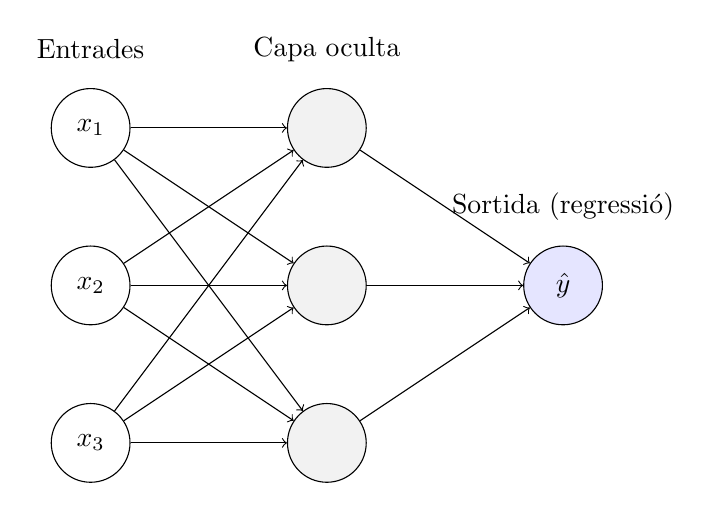
\begin{tikzpicture}[scale=1, transform shape]

% Input layer
\node[circle, draw, minimum size=1cm] (I1) at (0,2) {$x_1$};
\node[circle, draw, minimum size=1cm] (I2) at (0,0) {$x_2$};
\node[circle, draw, minimum size=1cm] (I3) at (0,-2) {$x_3$};

% Hidden layer
\node[circle, draw, fill=gray!10, minimum size=1cm] (H1) at (3,2) {};
\node[circle, draw, fill=gray!10, minimum size=1cm] (H2) at (3,0) {};
\node[circle, draw, fill=gray!10, minimum size=1cm] (H3) at (3,-2) {};

% Output layer
\node[circle, draw, fill=blue!10, minimum size=1cm] (O1) at (6,0) {$\hat{y}$};

% Connections input -> hidden
\foreach \i in {1,2,3}
  \foreach \h in {1,2,3}
    \draw[->] (I\i) -- (H\h);

% Connections hidden -> output
\foreach \h in {1,2,3}
  \draw[->] (H\h) -- (O1);

% Labels
\node at (0,3) {Entrades};
\node at (3,3) {Capa oculta};
\node at (6,1) {Sortida (regressió)};

\end{tikzpicture}
\caption{Esquema d’una xarxa neuronal de regressió}
\end{figure}

\section{Xarxa Neuronal amb llenguatge de programació}\label{sec:10}
En aquest apartat explicarem pas a pas de com vam crear el nostre xarxa neuronal de regressió.

\subsection{De celcius a fahrenheit}

Abans de començar a treballar amb la xarxa neuronal definitiu, vaig voler fer una més simple per tal de coneixer amb més profunditat de com funciona una xarxa neuronal de regressió; en aquest cas he escollit un transformador d'unitats de temperatura, de celcius (Unitat de temperatura basada en el punt de fusió de l'aigua) a fahrenheit (sistema d'unitat basada en el punt d'ebullició i solidificació de l'aigua). Per crear aquesta xarxa vaig escollir el Python com a llenguatge de programació, i el motiu esta explicat en l'apartat \ref{sec:4.4}.

\begin{figure}[H]
    \centering
    \includegraphics[width=0.5\textwidth]{./figures/1.png}
    \caption{biblioteques del Python}
\end{figure}

Per començar a crear una xarxa neuronal lo primer que s'ha de fer es importar totes les biblioteques necessaries per el treball. En aquest cas he importat els biblioteques tensorflow i numpy, com podeu veure també he posat un as per transformar les nominacions de les biblioteques en abrevació.
\begin{itemize}
 \item \textbf{tensorflow: }
 \item \textbf{numpy: }
\end{itemize}














font(\href{https://www.youtube.com/watch?v=iX_on3VxZzkhttps://www.youtube.com/watch?v=iX_on3VxZzk}{Xarxa neuronal amb Python})


















\section{Xarxa Neuronal amb fulls de calculs}\label{sec:11}
En aquest apartat continuarem amb la xarxa neuranal de regressió però aquesta vegada utilizarem un full de calculs per fer-ho.

\section{Comparació entre una xarxa neurnal creada per un llenguatge de programació netre una de fulls de calculs}

\section{Xarxa Neuronal amb un cas real}\label{sec:12}
